\documentclass[tikz,border=5pt]{standalone}
\usepackage[T1]{fontenc}
\usepackage{fix-cm}
\definecolor{friendlyA}{RGB}{128, 224, 255}
\definecolor{hostileA}{RGB}{255, 128, 128}
\definecolor{neutralA}{RGB}{170, 255, 170}
\definecolor{unknownA}{RGB}{255, 255, 128}
\usetikzlibrary{shapes.geometric, positioning}

\begin{document}

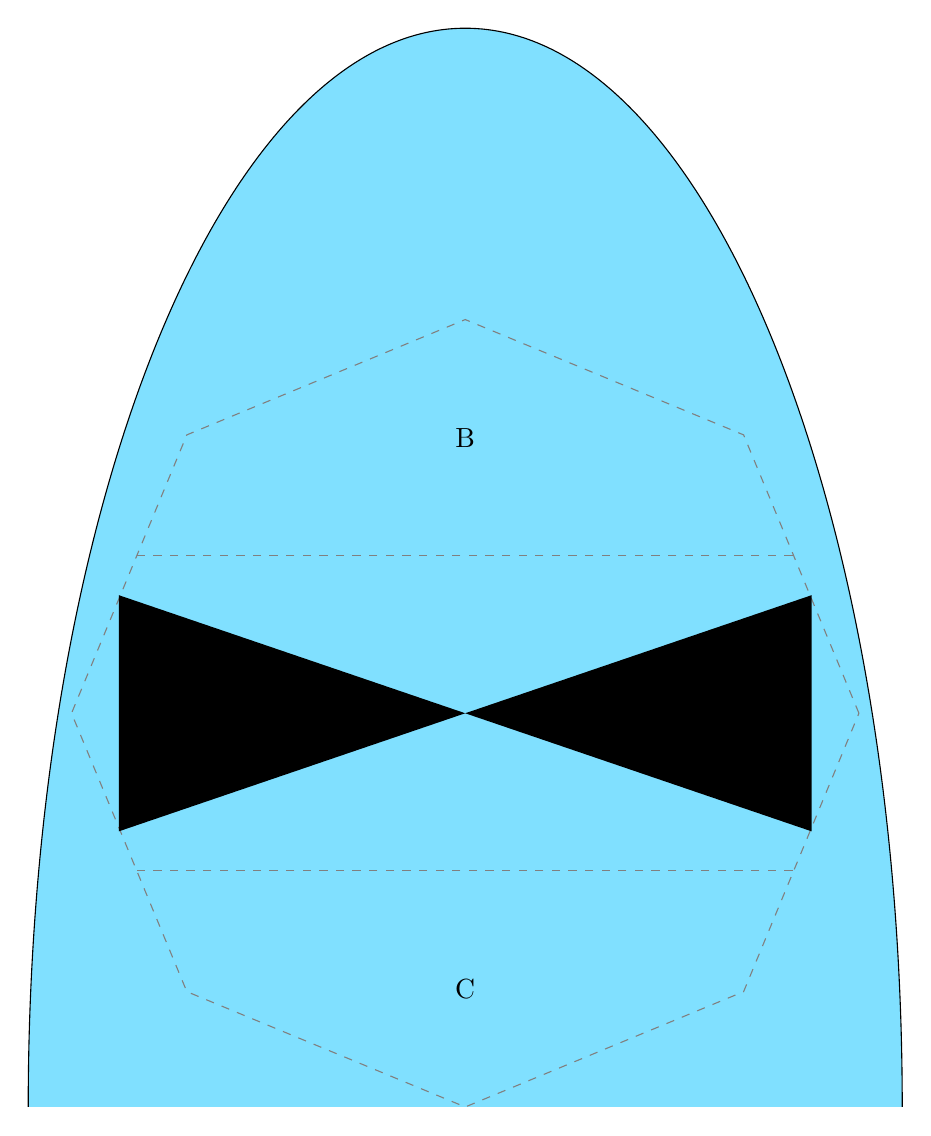
\begin{tikzpicture}[scale=10]

\draw[fill=friendlyA] (-0.555, -0.5) arc (180:0:0.555 and 1.37);

%\draw[fill=hostileA] (0.5, -0.5) -- (0.5, 0.21) -- (0, 0.71) --  (-0.5, 0.21) --  (-0.5, -0.5);

%\draw[fill=neutralA] (0.5, -0.5) -- (0.5, 0.5) -- (-0.5, 0.5) -- (-0.5, -0.5);

%\draw[fill=unknownA] (315:0.5) arc (-90:90: 0.354);
%
%\begin{scope}[rotate=90]
%	\draw[fill=unknownA] (315:0.5) arc (-90:90: 0.354);
%\end{scope}
%
%\begin{scope}[rotate=180]
%	\draw[fill=unknownA] (315:0.5) arc (-90:90: 0.354);
%\end{scope}
%
%\fill[unknownA] (315:0.5) -- (45:0.5) -- (135:0.5) -- (225:0.5) -- cycle; 


\draw[gray, dashed] (0:0.5) -- (45:0.5) -- (90:0.5) -- (135:0.5) -- (180:0.5) -- (225:0.5) -- (270:0.5) -- (315:0.5) -- cycle;
\begin{scope}
\clip (0:0.5) -- (45:0.5) -- (90:0.5) -- (135:0.5) -- (180:0.5) -- (225:0.5) -- (270:0.5) -- (315:0.5) -- cycle;
	\draw[gray, dashed] (0.5, 0.2) -- (-0.5, 0.2);
	\draw[gray, dashed] (0.5, -0.2) -- (-0.5, -0.2);
\end{scope}

%\node at (0,0) {A};
\node at (0,0.35) {B};
\node at (0,-0.35) {C};

\fontfamily{phv}\fontseries{bx}\selectfont \fontsize{100}{0}\selectfont

%%% MILITARY
%\node at (0,0) {MIL}; 

%%% CIVILIAN
%\node at (0,0) {CIV}; 

%%% MILITARY FIXED WING

%\fill (-0.36,0.125) arc (77:275:0.075 and 0.125) -- (0,0) -- cycle;
%
%\begin{scope}[xscale=-1]
%\fill (-0.36,0.125) arc (77:275:0.075 and 0.125) -- (0,0) -- cycle;
%\end{scope}

%%% CIVILIAN FIXED WING

%\draw (-0.36,0.125) arc (77:275:0.075 and 0.125) -- (0,0) -- cycle;
%
%\begin{scope}[xscale=-1]
%\draw (-0.36,0.125) arc (77:275:0.075 and 0.125) -- (0,0) -- cycle;
%\end{scope}


%%% MILITARY ROTARY WING

\fill (0.44, 0.15) -- (0.44, -0.15) -- (-0.44, 0.15) -- (-0.44, -0.15) -- cycle;

%%% CIVILIAN ROTARY WING

%\draw (0.44, 0.15) -- (0.44, -0.15) -- (-0.44, 0.15) -- (-0.44, -0.15) -- cycle;

%%% MILITARY BALLOON

%\fill (0, 0.025) circle (0.175);
%\fill (-0.05, 0) -- (-0.05,-0.2) -- (0.05, -0.2) -- (0.05,0) -- cycle;

%%% CIVILIAN BALLOON

%\draw (0, 0.025) circle (0.175);
%\begin{scope}
%
%\tikzstyle{reverseclip}=[insert path={(current bounding box.north east) --
%  (current bounding box.south east) --
%  (current bounding box.south west) --
%  (current bounding box.north west) --
%  (current bounding box.north east)}
%]
%
%\clip (0, 0.025) circle (0.175) [reverseclip];
%	\draw (-0.05, 0) -- (-0.05,-0.2) -- (0.05, -0.2) -- (0.05,0) -- cycle;
%\end{scope}

%%% MILITARY AIRSHIP

%\fill (0, 0) ellipse (0.45 and 0.15);
%\fill (0.2, 0) -- (0.3, 0.175) -- (0.4,0.175) -- (0.375,0) -- (0.4,-0.175) -- (0.3, -0.175) -- cycle;

%%% CIVILIAN AIRSHIP

%\draw (0, 0) ellipse (0.45 and 0.15);
%\begin{scope}
%
%\tikzstyle{reverseclip}=[insert path={(current bounding box.north east) --
%  (current bounding box.south east) --
%  (current bounding box.south west) --
%  (current bounding box.north west) --
%  (current bounding box.north east)}
%]
%
%\clip (0, 0) ellipse (0.45 and 0.15) [reverseclip];
%	\draw (0.2, 0) -- (0.3, 0.175) -- (0.4,0.175) -- (0.375,0) -- (0.4,-0.175) -- (0.3, -0.175) -- cycle;
%\end{scope}

%%% UAV

%\fill (0, -0.1) -- (0.45, 0.05) -- (0.45,0.1) -- (0, 0.025) -- (-0.45, 0.1) -- (-0.45, 0.05) -- cycle;

%%% AIR DECOY

%\fill (0.42, -0.2) -- (0.42, -0.175) --  (-0.42, -0.175) --  (-0.42, -0.2) -- cycle;
%
%\begin{scope}[shift={(-0.18,0)}]
%	\fill (-0.24, 0.025) -- (-0.0, 0.2) -- (-0.0, -0.15) -- cycle;
%\end{scope}
%
%\begin{scope}[shift={(0.12,0)}]
%	\fill (-0.24, 0.025) -- (-0.0, 0.2) -- (-0.0, -0.15) -- cycle;
%\end{scope}
%
%\begin{scope}[shift={(0.42,0)}]
%	\fill (-0.24, 0.025) -- (-0.0, 0.2) -- (-0.0, -0.15) -- cycle;
%\end{scope}


%%% MEDIC

%\fill (-0.075, -0.2) -- (0.075, -0.2) -- (0.075, 0.2) -- (-0.075, 0.2) -- cycle;
%
%\begin{scope}[rotate=90]
%\fill (-0.075, -0.2) -- (0.075, -0.2) -- (0.075, 0.2) -- (-0.075, 0.2) -- cycle;
%\end{scope}

%%% ATTACK/STRIKE

%\node at (0,0) {A}; 

%%% BOMBER

%\node at (0,0) {B};

%%% CARGO

%\node at (0,0) {C};

%%% FIGHTER

%\node at (0,0) {F}; 

%%% JAMMER / ECM

%\node at (0,0) {J}; 

%%% TANKER

%\node at (0,0) {K}; 

%%% PATROL

%\node at (0,0) {P};  
 
%%% RECON

%\node at (0,0) {R};

%%% TRAINER

%\node at (0,0) {T};

%%% UTIL

%\node at (0,0) {U};

%%% VSTOL

%\node at (0,0) {V};

%%% ACP

%\node at (0,0) {ACP};

%%% AEW

%\node at (0,0) {AEW}; 

%%% ASUW

%\node at (0,0) [xscale=0.75] {ASUW};      

%%% ASW

%\node at (0,0) {ASW}; 

%%% COM

%\node at (0,0) {COM}; 

%%% CSAR

%\node at (0,0) [xscale=0.75] {CSAR};

%%% ESM

%\node at (0,0) {ESM};       

%%% GOV

%\node at (0,0) {GOV};

%%% MCM

%\node at (0,0) {MCM};

%%% PR

%\node at (0,0) {PR};       
       
%%% PX

%\node at (0,0) {PX};       
       
%%% SAR

%\node at (0,0) {SAR};

%%% SEAD

%\node at (0,0) [xscale=0.75] {SEAD};

%%% SOF

%\node at (0,0) {SOF};

%%% UL

%\node at (0,0) {UL};

%%% R

%\node at (0,0) {R};

%%% VIP

%\node at (0,0) {VIP};                     
       
       



\end{tikzpicture}

\end{document}
